{\color{indiagreen}\subsection{Kroženje}}
\textbf{ENAKOMERNO}
\begin{center}
	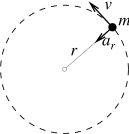
\includegraphics[width=7cm, height=7cm,keepaspectratio=true]{Krozenje.png}
\end{center}
Kroženje je vedno pospešeno gibanje saj se \textbf{vektor vedno spreminja}. Enakomerno pa ker je \textbf{$|\vec{v}|$ vedno konstanten}, ne pa sam $\vec{v}$.\\
$t_0$ - obhodni čas.\\
$\nu$ - frekvenca, predstavi število obratov v nekem času.\\
\begin{align*}
	\nu &= \frac{N}{t} = \frac{1}{t_0} [Hz] 
\end{align*}
$\omega$ - kotna hitrost, pove nam za kakšen kot prepotujemo v določenem času, enote so v radianih na sekundo\\
\begin{align*}
	v &= \frac{\Delta \phi}{\Delta t} = \frac{360^{\circ}}{t_0} = \frac{2\pi}{t_0} = 2\pi\frac{1}{t_0} = {\color{bostonuniversityred}2\pi\nu} [\frac{1}{s}] 
\end{align*}
v - ubodna histrost, je tangentan na krožnico, ubod pomeni zunanji rob, pove nam kolikšen krožni lok(odsek krožnice opravi v določenem času).\\
\begin{align*}
	v &= \frac{\Delta l}{\Delta t} = {\color{bostonuniversityred}\frac{2\pi r}{t_0}} = 2\pi \frac{1}{t_0} r = {\color{bostonuniversityred}\omega r} [\frac{m}{s}] 
\end{align*}
$a_r$ - radialni pospešek, cedno kaže v središče, spreminja smer hitrosti na krožnici.\\
\begin{align*}
	a_r &= \frac{\Delta v}{\Delta t} = {\color{bostonuniversityred}v\omega = r\omega^2 = \frac{v^2}{r}} [\frac{m}{s^2}] 
\end{align*}
